\documentclass[12pt,a4paper]{article}

\usepackage[UTF8]{ctex}
\usepackage{amsmath,amscd,amsbsy,amssymb,latexsym,url,bm,amsthm}
\usepackage{amsfonts}
\usepackage{epsfig,graphicx,subfigure}
\usepackage{hyperref}
\usepackage{listings}
\usepackage[vlined,ruled,linesnumbered]{algorithm2e}
\usepackage{enumitem}
\usepackage{xcolor}
\usepackage{geometry}

%\uppercase\expandafter{\romannumeral1}:% 罗马数字。

\lstset{
language=Matlab,
keywordstyle= \color{blue!70},
commentstyle= \color{red!50!green!50!blue!50},
breaklines
}%设置listing插入语言

\setlength{\parindent}{0em}
\setlength{\parskip}{1em}

\geometry{bottom =3cm}
\newcommand{\textbi}[1]{%
\textbf{\textit{#1}}}

\newcommand{\ncolor}[1]{%
{\color[RGB]{139,117,0}{#1}}}
\newtheorem{theorem}{Theorem}[section]
\newenvironment{solution}{{\noindent \it \textbf{Solution:}}\\}

\title{Evaluation model}
\author{Yunlong Cheng}

\begin{document}
\maketitle
\section{主成分分析(PCA)}
\subsection{简单实例}
由一组数据如下:
\begin{center}
  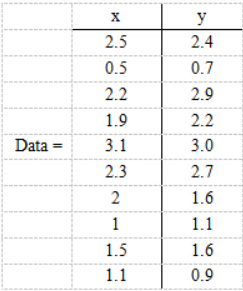
\includegraphics[width = 0.25\textwidth]{figures/simple_data.png}
\end{center}
行代表案例,列代表特征,这里有10个案例,两个特征。

分析:
\begin{enumerate}
  \item 第一步:求 $x$ 和 $y$ 的平均值,对于所有案例减去平均值,得:
  \begin{center}
    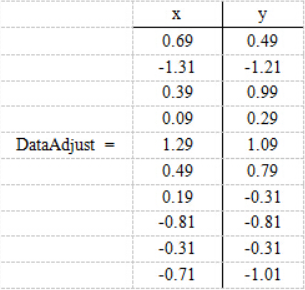
\includegraphics[width = 0.25\textwidth]{figures/simple_data_adjust.png}
  \end{center}
  \item 第二步:求特征协方差矩阵,在这里为
  \begin{equation*}
    cov = \left(
    \begin{array}{cc}
      .6165 & .6154 \\
      .6154 & .7165 \\
    \end{array}\right)
  \end{equation*}
  \item 第三步,求协方差的特征值和特征向量:
  $$eginvalues = \binom{.04908}{1.28402}$$
  \begin{equation*}
    eginvectors = \left(
    \begin{array}{cc}
      -.7351 & -.6678\\
      .6678 & -.7351\\
    \end{array}\right)
  \end{equation*}
  \item 第四步,将特征值从大到小排序,选择其中最大的 $k$ 个。在这里我们选择 $1.28402$,特征向量为 $\binom{-.6678}{-.7351}$.
  \item 第五步,将样本点投影到选取的特征向量上,投影后的数据为:
  \begin{center}
    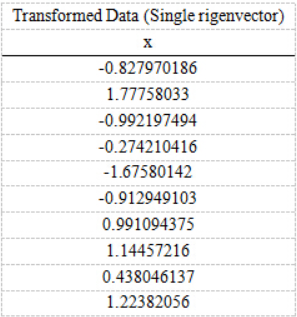
\includegraphics[width = 0.3\textwidth]{figures/simple_transdata.png}
  \end{center}
\end{enumerate}

\section{理想解方法 (TOPSIS)}
问题:

为了客观地评价我国研究生教育的实际状况和各研究生院的教学质量,国务院学位委员会办公室组织过一次研究生院的评估。为了取得经验,先选5所研究生院,收集有关数据资料进行了试评估,下表是所给出的部分数据:
\begin{center}
  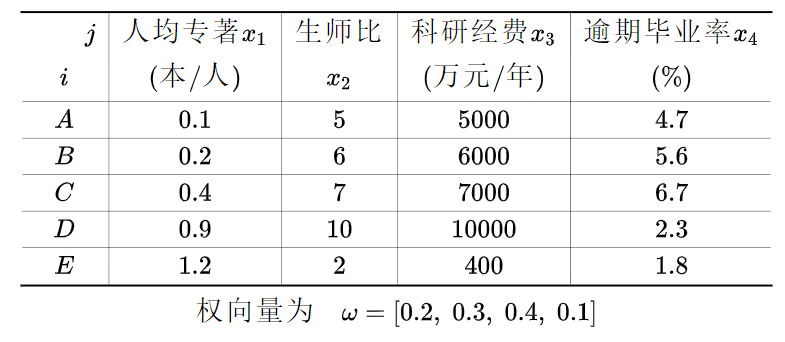
\includegraphics[width = 0.8\textwidth]{figures/topsis_data.png}
\end{center}
解:
\begin{enumerate}
  \item 指标同向化处理:因为有的指标是越小越好,有的指标是越大越好,同向化消除这些影响。
  \begin{itemize}
    \item 人均专著、科研经费为效应型指标(越大越好)
    \item 逾期毕业率为成本型指标(越小越好)
    \item 生师比为区间型指标
  \end{itemize}
  \begin{center}
    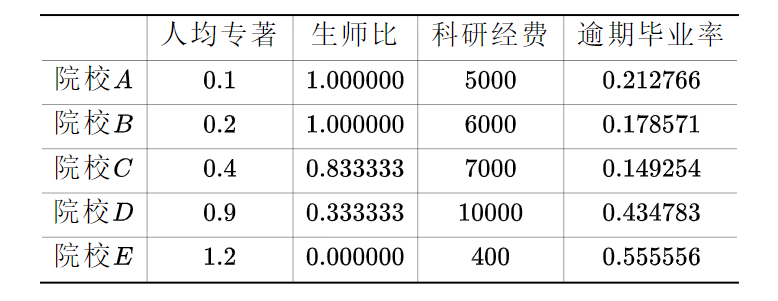
\includegraphics[width = 0.8\textwidth]{figures/topsis_samedir.png}
  \end{center}
  \item 构造归一化矩阵:
  例:院校 A 的人均专属:$\frac{0.1}{\sqrt{0.1^2+0.2^2+0.4^2+0.9^2+1.2^2}} = 0.0637$
  得:
  \begin{center}
    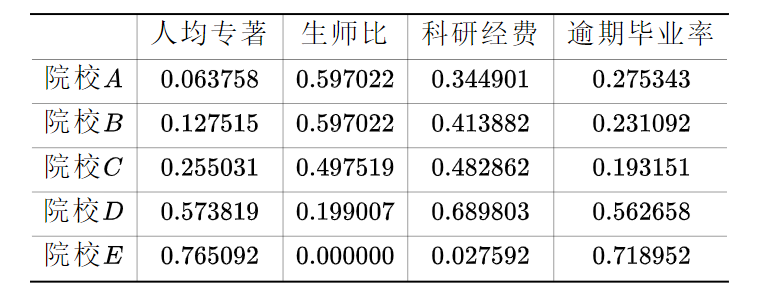
\includegraphics[width = 0.8\textwidth]{figures/topsis_normalization.png}
  \end{center}
  \item 构造加权规范阵:$c_{ij} = w_{ij}\cdot b_{ij}$。
  \item 确定正理想解 $C^*$ 和负理想解 $C^0$
  \begin{center}
    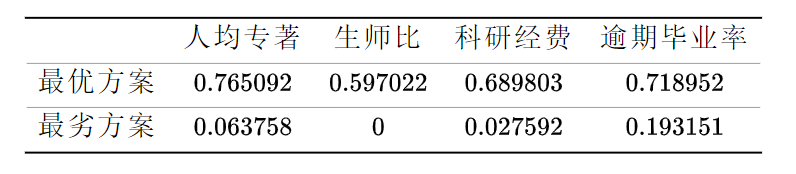
\includegraphics[width = 0.8\textwidth]{figures/topsis_idealsol.png}
  \end{center}
  \item 计算各方案到正理想解与负理想解的距离:
  \begin{itemize}
    \item 到正理想解的距离为:$s_i^*$
    \item 到负理想解的距离为:$s_i^0$
  \end{itemize}
  \item 计算各方案的排序指标值(综合评价指数):
  $$f_i^* = \frac{s_i^0}{s_i^0 + s_i^*}\quad i = 1, 2, \cdots ,m$$
  \begin{center}
    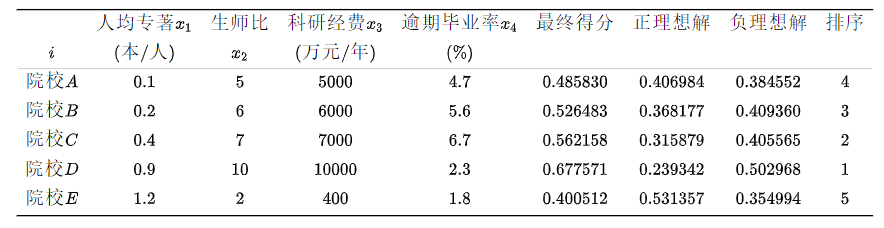
\includegraphics[width = 0.9\textwidth]{figures/topsis_finalresult.png}
  \end{center}
\end{enumerate}

\section{熵权法}
问题:

某医院为了提高自身的护理水平,对拥有的11个科室进行了考核,考核标准包括9项整体护理,并对护理水平较好的科室进行奖励。下表是对各个科室指标考核后的评分结果。
\begin{center}
  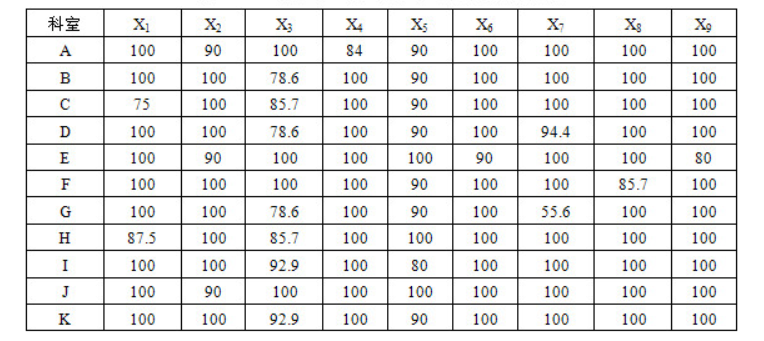
\includegraphics[width = \textwidth]{figures/entropy_data.png}
\end{center}
解:
\begin{enumerate}
  \item 对原始数据进行归一化:
  $y_{ij} = \frac{x_{ij} - \min(X_j)}{\max(X_j) - \min(X_j)}$
  \begin{center}
    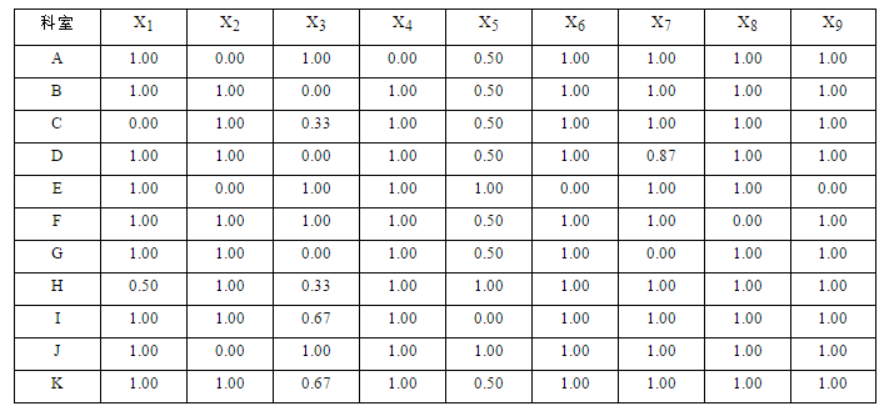
\includegraphics[width = 0.9\textwidth]{figures/entropy_adjdata.png}
  \end{center}
  \item 求信息熵:
  $$p_{ij} = \frac{t_{ij}}{\sum_{i = 1}^ny_{ij}}\quad\quad E_{ij} = -\sum_{i = 1}^np_{ij}log_nP_{ij}$$
  \begin{center}
    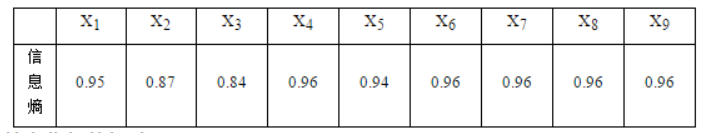
\includegraphics[width = 0.9\textwidth]{figures/entropy_entropy.png}
  \end{center}
  \item 确定各指标信息熵权重:
  $$W_j = \frac{1 - E_{j}}{\sum_{j = 1}^n(1 - E_j)}$$
  \begin{center}
    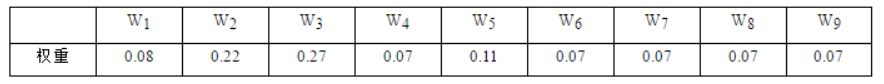
\includegraphics[width = 0.9\textwidth]{figures/entropy_weight.png}
  \end{center}
  \item 对各个科室进行评分:
  $$a_i = \sum_{j = 1}^kW_jx_{ij}\quad (i = 1, 2, \cdots ,n)$$
  \begin{center}
    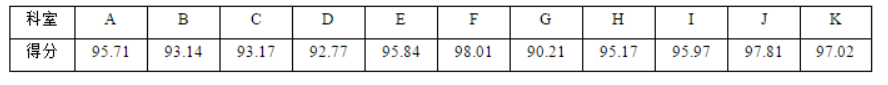
\includegraphics[width = 0.9\textwidth]{figures/entropy_finalresult.png}
  \end{center}


\end{enumerate}



\end{document}
